%----------------------------------------------------------------------------------------
% PACKAGES AND DOCUMENT CONFIGURATIONS
%----------------------------------------------------------------------------------------

  \documentclass[12pt]{article}

  \usepackage{hyperref}
  \usepackage{fancyhdr} % Required for custom headers
  \usepackage{lastpage} % Required to determine the last page for the footer
  \usepackage{extramarks} % Required for headers and footers
  \usepackage[usenames,dvipsnames]{color} % Required for custom colors
  \usepackage{graphicx} % Required to insert images
  \usepackage{listings} % Required for insertion of code
  \usepackage{courier} % Required for the courier font
  \usepackage{lipsum} % Used for inserting dummy 'Lorem ipsum' text into the template
  \usepackage{wrapfig}
  \usepackage{color}
  \usepackage{lscape}

  \setlength\parindent{0pt} % Removes all indentation from paragraphs
  \renewcommand{\labelenumi}{\alph{enumi}.} % Make numbering in the itemize environment by letter rather than number (e.g. section 6)
  \lstset{basicstyle=\ttfamily\footnotesize,breaklines=true}

  % Margins
  \topmargin=-0.4in
  \evensidemargin=0.2in
  \oddsidemargin=-0.2in
  \textwidth=7.0in
  \textheight=9.0in
  % \headsep=0.25in

  % \linespread{1.1} % Line spacing

  \definecolor{dkgreen}{rgb}{0,0.6,0}
  \definecolor{gray}{rgb}{0.5,0.5,0.5}
  \definecolor{mauve}{rgb}{0.58,0,0.82}
  \definecolor{greyish}{rgb}{0.96,0.96,0.96}

  \lstset{
    backgroundcolor=\color{greyish},   % choose the background color; you must add \usepackage{color} or \usepackage{xcolor}
    frame=tblr,
    numbers=left,                       % where to put the line-numbers; possible values are (none, left, right)
    numbersep=5pt,                   % how far the line-numbers are from the code
    numberstyle=\tiny\color{mygray}, % the style that is used for the line-numbers
    language=Ruby,
    aboveskip=3mm,
    belowskip=3mm,
    showstringspaces=false,
    columns=flexible,
    basicstyle={\footnotesize\ttfamily},
    numbers=none,
    numberstyle=\tiny\color{gray},
    keywordstyle=\color{blue},
    commentstyle=\color{dkgreen},
    stringstyle=\color{mauve},
    breaklines=true,
    breakatwhitespace=true
    tabsize=1
  }

  \begin{document}
  \begin{titlepage}

%----------------------------------------------------------------------------------------
% TITLE PAGE INFORMATION
%----------------------------------------------------------------------------------------
 \newcommand{\HRule}{\rule{\linewidth}{0.5mm}} % Defines a new command for the horizontal lines, change thickness here
  \begin{center} % Center everything on the page

  %----------------------------------------------------------------------------------------
  % HEADING SECTIONS
  %----------------------------------------------------------------------------------------
  \textsc{\large Faculty of Computers, Informatics and Microelectronics}\\[0.5cm]
  \textsc{\large Technical University of Moldova}\\[1.2cm] % Name of your university/college
  \vspace{35 mm}
  \textsc{\Large PAD}\\[0.5cm] % Major heading such as course name
  %\textsc{\large Laboratory work \#1-3}\\[0.5cm] % Minor heading such as course title
  \textsc{\large Laboratory work \# 4,5}\\[0.5cm] % Minor heading such as course title

  %----------------------------------------------------------------------------------------
  % TITLE SECTION
  %----------------------------------------------------------------------------------------
  \vspace{10 mm}
  \HRule \\[0.4cm]
  { \large \bfseries  Processing and distribution of xml and json data.\\ Validation of xml data}\\[0.4cm] % Title of your document
  \HRule \\[1.5cm]

  %----------------------------------------------------------------------------------------
  % AUTHOR SECTION
  %----------------------------------------------------------------------------------------
      \vspace{25mm}

      \begin{minipage}{0.4\textwidth}
      \begin{flushleft} \large
      \emph{Authors:}\\
      \textbf{Petru \textsc{Negrei}} \\
      Victor \textsc{Vasilica}
      \end{flushleft}
      \end{minipage}
      ~
      \begin{minipage}{0.4\textwidth}
      \begin{flushright} \large
      \emph{Supervisor:} \\
      D. \textsc{Ciorba} % Supervisor's Name
      \end{flushright}
      \end{minipage}\\[4cm]

      \vspace{5 mm}
      % If you don't want a supervisor, uncomment the two lines below and remove the section above
      %\Large \emph{Author:}\\
      %John \textsc{Smith}\\[3cm] % Your name

      %----------------------------------------------------------------------------------------
      % DATE SECTION
      %----------------------------------------------------------------------------------------

      {\large November 2014}\\[3cm] % Date, change the \today to a set date if you want to be precise

      %----------------------------------------------------------------------------------------
      % LOGO SECTION
      %----------------------------------------------------------------------------------------

      %\includegraphics{Logo}\\[1cm] % Include a department/university logo - this will require the graphicx package

      %----------------------------------------------------------------------------------------

      \vfill % Fill the rest of the page with whitespace
      \end{center}
      \end{titlepage}

      % \newpage
      % \tableofcontents
      % \newpage

%----------------------------------------------------------------------------------------
% Introduction
%----------------------------------------------------------------------------------------

  \section{Introduction}

  \subsection{Topic}

  Processing and distribution of xml and json data.

  \subsection{Objective}

  The aim of the laboratory work lies in the study of models for processing XML data (DOM / SAX) and JSON to distribution.

  \subsection{Generic requirements}

  \subsubsection{Task}

  Develop a system of distributed heterogeneous data, centralized in one node type warehousing.

  \subsubsection{Report}

  Report will contain a short description of work done, and will present necesary information
  about tools, algorithms used or studied.

%----------------------------------------------------------------------------------------
% Implementation
%----------------------------------------------------------------------------------------
  
  \section{Structure}

    Below you can see the structure of the application, there are represented the classes used 
    and their variables and methods. The application is composed of three main clasess \textit{Client}
    and \textit{Server} and \textit{Main Server}. \\

    The \textit{Client} and \textit{Server} classes use the \textit{HttpHandler} helper class in order to
    send the necesary requests to the \textit{Main Server} and also recieve the response from it. \\ 

    The requests are handled and analyzed on \textit{Main Server} in different threads and saved on 
    a single file, the server doesn't duplicate the records it already has them in his json database file, 
    for this it uses an additional \textit{Hash} file that saves the messages received in a Hash format. 

    \begin{minipage}[b]{1.0\linewidth}
      \begin{center}
        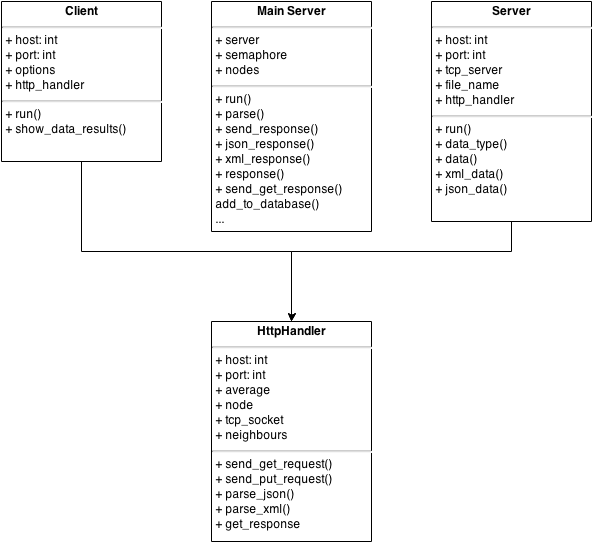
\includegraphics[width=0.65\textwidth]{diagram}
         \\ Fig. 1 Class diagram
      \end{center}
    \end{minipage}
    
  \section{Implementation}

    \subsection{Main server}

    The most important function of the main server is to receive different request, and 
    depending on type and parameters of request to perform certain actions.  \\

    The \textit{run} function is the function that receives requests from nodes or
    client in a thread safe way and depending of the type of request it acess different 
    methods. 

    \begin{lstlisting}
    # ...
     def run
        loop do
         Thread.start(server.accept) do |client|
            @semaphore.synchronize do
              request = client.gets
              request =~ /^GET.*/ ? send_response(client, request) : add_to_database(client.read)
              client.close
            end
          end
        end
      end
    # ... 
    \end{lstlisting}

    Below I will describe how the \textit{GET} sequence it is executed. The \textit{PUT} request 
    processing was implemented and described by my colegue.  \\ 

    The first function that is accessed is 

    \begin{itemize}
      \renewcommand{\labelitemi}{$\circ$}
      \item \textit{send\_response} - the method that sends data depending on the type of request received.
      \item \textit{json\_response} - returns the json response. 
      \item \textit{xml\_response} - returns the xml response.
      \item \textit{response} - the method that returns the data depending of the user request.
      \item \textit{send\_get\_response} -  sends the response in the right format with the right data.
    \end{itemize}

    \begin{lstlisting}
     # ... 
     def send_response client, request
      @header, _, type = parse_request(request << client.gets)
      type == 'json' ? send_get_response(client, json_response) : send_get_response(client, xml_response)
     end

     def json_response
        JSON.generate  response
      end

      def xml_response
        response.to_xml(:root => 'employees')
      end

      # needs refactor, bad implementation
      def response
        id = @header.scan(/\d+/)
        if id.empty? 
          current_employees 
        else
          (current_employees.size < id.first.to_i-1) ? {"problem" => "There is no such id" } : current_employees[id.first.to_i-1]
        end
      end

      def send_get_response client, response
         client.print "HTTP/1.1 200 OK\r\n" +
                "Content-Type: text/plain\r\n" +
                "Content-Length: #{response.bytesize}\r\n" +
                "Connection: close\r\n"

        client.print "\r\n"
        client.print response
        client.close
      end
      # ...
    \end{lstlisting}

    \subsection{Client Side}

    The client side suffered a small number of modifications compared to previous versions, 
    because the all the necessary data is received with \textit{GET} request, there is no need
    to establish a TCP connection with other nodes to get the data. 

    \subsubsection{HTTP Handler}

    The handler permforms the same functions that it done previously but with some adjustments.

    \begin{itemize}
      \renewcommand{\labelitemi}{$\circ$}
      \item \textit{send\_get\_request} - method that will send get request that contains the type.
      \item \textit{get\_response} - method that receives the \textit{GET} response from the main server.
      \item \textit{parse\_json} - parse the response with json.
      \item \textit{parse\_xml} - parses the xml response with json.
    \end{itemize}

    \begin{lstlisting}
    # ... 
      def send_get_request request, type
       header =["GET #{request} HTTP/1.0",
            "Accept-Type: application/#{type}"].join("\r\n")

        tcp_socket.puts header + "\r\n\r\n"    
        type == 'json' ? parse_json(get_response) : parse_xml(get_response)
      end

      def parse_json response
        p "Received json"
        @data = JSON.parse response
      end
      
      def parse_xml response
        p "Received xml"
        @data = JSON.parse(Hash.from_xml(response).to_json)
      end

      def get_response
        request = tcp_socket.read
        _, body = request.split("\r\n\r\n")
        tcp_socket.close
        body
      end
      # ...
    \end{lstlisting}

    \subsubsection{Data manipulation}

    Data manipulation class as the name says it responsible to analyze,
    parse and show received data in a readable form.

    \newpage

    \begin{itemize}
      \renewcommand{\labelitemi}{$\circ$}
      \item \textit{show\_all} - display all the employers received from \textit{GET} request.
      \item \textit{show\_entry}  - display the entry in a table format.
      \item \textit{table\_format} - add the table format to the parsed data.
      \item \textit{check\_xml?} - checks if received data was in xml format.
    \end{itemize}

    \begin{lstlisting}
    class DataManipulation
      # ... 
      def show_all
        @data = @data["employees"] if check_xml?
        puts table_format(data)
      end

      def show_entry
        @data = @data["employees"] if check_xml_entry?
        puts entry_table_format(data)
      end

      private

      def table_format data
        # ... 
      end

      def entry_table_format data
        # ... 
      end

      def check_xml?
        data.is_a? Hash
      end

      def check_xml_entry?
        data.has_key? "employees"
      end

  end
    \end{lstlisting}

    \subsubsection{Main}

    The main class \textit{Client} contains all methods that are necesary to start and perform necesary
    work. Below there is a short description of methods that it has, for the implementation you can see the full code.

    \begin{itemize}
      \renewcommand{\labelitemi}{$\circ$}
      \item In the \textit{contructor} we save provided options and setup http handler.
      \item \textit{run} - performs get request to the main server.
      \item \textit{show\_data\_results} - show data received from mian server, based on option from console.
    \end{itemize}

    \begin{lstlisting}
      class Client

        HOST = 'localhost'
        FILE_NAME = "client_data.json"

        attr_reader :http_client,  :options

        def initialize options
          @options = options
          @http_client = HttpHandler.new HOST, 8000
        end

        def run
          http_client.send_get_request options[:request], options[:type]
          show_data_results
        end

        private

        def show_data_results
          dt = DataManipulation.new(http_client.data)
          options[:request] =~ /\d+/ ? dt.show_entry : dt.show_all
        end

      end
    \end{lstlisting}

    The script receives two kind of arguments the request and the type of it.

    \begin{lstlisting}
    options = {}
    OptionParser.new do |opts|
      opts.banner =  "Usage: ruby client.rb [options]\n\n"
      opts.on("-r", "--request [request]", "get request to main server") do |request|
        options[:request] = request || "/emploees"
      end

      opts.on("-t", "--type [TYPE]", "file name containing data") do |type|
        options[:type] = type || "json"
      end
    end.parse!
    \end{lstlisting}

    The client actions are started with the following line, it receive
    the actions that need to be applied on the data.

    \begin{lstlisting}
    Client.new(options).run
    \end{lstlisting}

    \subsection{Server}

    The server part was done by Vasilica Victor and the handling of the \textit{PUT} requset on the main server.


    \subsection{Xml check}

    The nodes send the contents of their files with help of \textit{PUT} request, the \textit{Main Server} has the 
    functionality to check if the contents of the send message are valid and then save them into the file. \\ 

    First he loads the schema file of the xml that should match the xml it will receive.  

    \begin{lstlisting}
    @xml_schema = Nokogiri::XML::Schema(File.read("dataSchema.xsd"))
    \end{lstlisting}

    And the main check take place before saving to the database, it checks if the type is xml and then 
    validates with help of \textit{Nokogiri} librari with in case of errors will return an array of errors. Then
    we check if that array is empty then we pass the xml to json to our save method, otherwise the return
    a message of error to the terminal.

    \begin{lstlisting} 
     def add_to_database http_body
        _, _, type = parse_request http_header
        json = http_body

        if type == "xml"
          errors = xml_schema.validate(Nokogiri::XML(http_body))
          if errors.empty? #valid xml
            json = xml_to_json(http_body)
          else #invalid xml
            puts "ERROR: invalid xml"
            return
          end
        end
        save(json) unless check_uniq?(json)
      end
    \end{lstlisting}


    \section{Conclusion}

    In this laboratory work we build a distributed system that uses different type of data and different requests, each doing its own predefined task.
    Thus after learning more about the uses and formats of data, we apply each to solve their individual task. \\

    We build a helper class that handles all required requests \textit{GET} and \textit{PUT}, and receives the responses from the \textit{Main Server}.
    Depending on the request "/employess" or specific one "employees/id=1" and the type specified "json" or "xml", the \textit{Main Server} will 
    return the list of users or a single required user.

    We also worked with \textit{json} in order to store our collection of necesary data, on the \textit{Main Server} and also a array of hashes to prevent
    duplicated entries. 

    Thus we learned how to build a small distributed system with a collection of objects using different tpes and requests. \\

    \textbf{Link to Repository: } \url{https://gitlab.ati.utm.md/petru.negrei/lab4/tree/wip/petru}

   \section{References}

   \begin{itemize}
      \item Ruby Socket \url{http://www.ruby-doc.org/stdlib-1.9.3/libdoc/socket/rdoc/Socket.html}
      \item Ruby TCP  Socket \url{http://www.ruby-doc.org/stdlib-1.9.3/libdoc/socket/rdoc/TCPSocket.html}
      \item Ruby Mutex \url{http://wwwi.ruby-doc.org/core-2.1.4/Mutex.html}
      \item Ruby JSON \url{http://www.ruby-doc.org/stdlib-2.0.0/libdoc/json/rdoc/JSON.html}
      \item Ruby OptionParser \url{http://ruby-doc.org/stdlib-2.1.0/libdoc/optparse/rdoc/OptionParser.html}
   \end{itemize}

\end{document}